%!TEX root = ..\Master.tex

\section{Dimensionality Reduction}
\fixme{Remove this section from the report.}

%e.g. finding projection vectors, choosing number of components, applications.\\
%motivation:
%data compression
%speed up learning algorithm
When working with large amounts of data in higher dimensions you often need a lot of computing power. Dimensionality reduction is mostly used in order to speed up the learning algorithm. This section contains an explanation of two widely used dimensionality reduction methods, Principal component analysis (PCA) and Fisher Discriminant method (Fisher).


\subsection{PCA}

PCA is used for reducing the number of dimensions of a feature space.
It works by projecting the data in the feature space, down to a fewer dimensional feature space by minimizing the squared projection error.
The reduced feature space does not nessecarily share the same features, but new features are found which best retains the variance in the data.

PCA should mainly be used for compressing the data to save memory or reducing running time of learning algorithm.
By reducing the amount of features most machine learning algorithms runs faster.
PCA can also be used to prevent overfitting, but it is usually better to use regularization. \\

Figure \ref{fig:pca} shows a 3 dimensional feature space where all the data, within a small margin, lies in a 2 dimensional plane.
PCA is used to find two vectors $u^{(1)}$ and $u^{(2)}$ which spans this 2D plane.

\begin{figure}
\centering
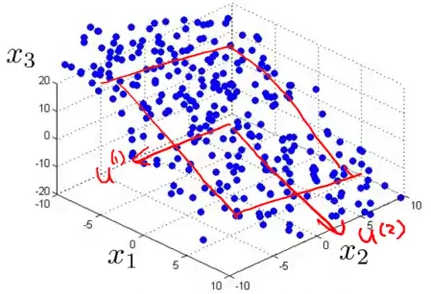
\includegraphics{images/pca}
\caption{3D to 2D PCA illustration}
\label{fig:pca}
\end{figure}

The plane is the 2 dimensions, in which the most variance is obtained in the data. Preprocessing of the data should be done before doing PCA. Given the training set:
\begin{equation}
x = 
\begin{bmatrix}
x_1 & x_2 & \dots & x_m
\end{bmatrix}
\end{equation}

Ensure that every feature has zero mean by doing mean normalization:
\begin{equation}
\mu_j = \frac{1}{m} \sum^m_{i=1} x_j^{(i)}
\end{equation}
\begin{equation}
x_j = x_j - \mu_j
\end{equation}

After preprocessing the data, we can do PCA on it. We start by computing the covariance matrix $\Sigma$:

\begin{equation}
\Sigma = \frac{1}{m} \sum^n_{i=1} x^{(i)} {x^{(i)}}^T
\end{equation}

The covariance matrix describes how the different features relates. When doing feature reduction we want to remove features which has high correlation with other features.
An example could be a feature which describes a length in cm and another feature describing the same length in inches.
These features will have very high correlation and one of them can be removed from the feature space without loosing much information. \\

Then we compute the eigenvectors of covariance matrix:
\begin{equation}
U = \begin{bmatrix}
   u^{(1)} & u^{(2)} & \dots & u^{(n)}
 \end{bmatrix}
\in \mathbb{R}^{n \times n}
\end{equation}

The eigenvectors will lay in the directions of most variance in the data. This is what is shown on Figure \ref{fig:pca}.
The longer the eigenvector, the more variance it describes.
Therefore we want to keep the longest eigenvectors and remove the shortest eigenvectors. The eigenvectors are ordered by length in the matrix $U$.  We select the first $k$ eigenvectors to get the reduced set of eigenvectors:

\begin{equation}
U_{reduce} = \begin{bmatrix}
   u^{(1)} & u^{(2)} & \dots & u^{(k)}
 \end{bmatrix}
\end{equation}

We can now calculate the new feature vectors:
\begin{equation}
z = U_{reduce}^Tx
\end{equation}

We have now reduced the feature space to a $k$ dimensional feature space.
Say we want to retain at least $95\%$ of the variance in the data.
We do this by picking the smallest value of $k$ so that:
\begin{equation}
\frac{\displaystyle\sum^{k}_{i=1} S_{ii}}{\displaystyle\sum^{n}_{i=1} S_{ii}} \geq 0.95
\end{equation}

The matrix $S$ is found by doing singular value decomposition (SVD). The matrix $S$ has the form:
\begin{equation}
S =  
\begin{bmatrix}
S_{11} & 0 & 0 & 0 & 0 \\
0 & S_{22} & 0 & 0 & 0 \\
0 & 0 & S_{33} & 0 & 0 \\
0 & 0 & 0 & \dots & 0 \\
0 & 0 & 0 & 0 & S_{nn} \\
\end{bmatrix}
\end{equation}

In our project we use PCA to reduce our feature space from 64 dimensions down to 40 dimensions.
We do this to increase the speed of our learning algorithms while still retaining almost all of our data ($\geq 99.99\%$) as seen on Figure \ref{fig:pca-on-our-data}.

\begin{figure}
\centering
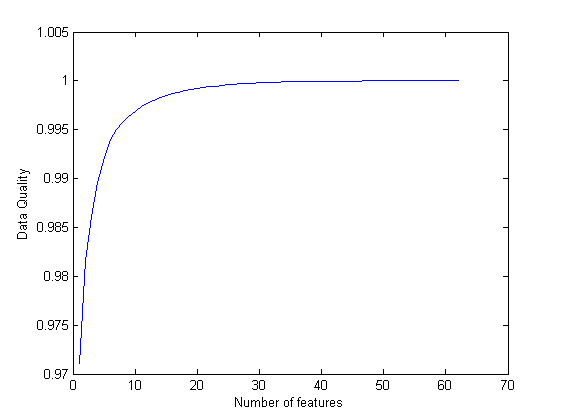
\includegraphics[scale = 0.8]{images/pca-on-our-data}
\caption{ Retained variance per dimension}
\label{fig:pca-on-our-data}
\end{figure}

\subsection{Fisher}
Fisher's linear discriminant is another look on dimensionality reduction. Instead of maximizing the variance of the data, we use the information we have on the classes to separate them as much as possible. We use equation \ref{fisher1} and place a threshold on y such that class 1: $y\geqslant -\omega_0$ and class 2 is everything else. This is also said as projecting data down to one dimension.
\begin{equation}
\label{fisher1}
y = \textbf{w}^T\textbf{x}
\end{equation}
This leads to a considerable loss in information and may cause overlapping in data that did not overlap in multidimensional space as can be see on figure \ref{fig:fisher} from the book Pattern Recognition and Machine Learning by Christopher M. Bishop\cite{bishop2006pattern}. The left Image is  the original space while the right image is in the projected space.\\
\begin{figure}
\centering
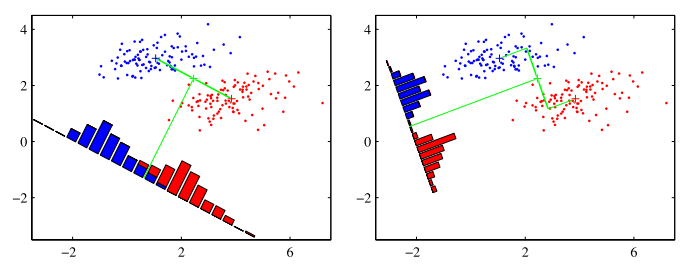
\includegraphics[width=1\textwidth]{images/fisher}
\caption{Picture from the Pattern Recognition and Machine Learning Book by Christopher M. Bishop}
\label{fig:fisher}
\end{figure}
By adjusting the weight vector \textbf{w} a solution can be found that minimises overlapping by maximising the distance between classes. Given two classes we have:
\begin{equation}
m_1 = \frac{1}{N_1} \sum_{n=C_1} X_n,       m_2 = \frac{1}{N_2} \sum_{n=C_2} X_n
\end{equation}
With \textbf{m} being the mean of the class and \texttt{N} being the amount of points in the class. The goal is to maximise the difference $m_2 - m_1$ and this is done by maximising the difference of the projected data as well:
\begin{equation}
m_2 - m_1 = \textbf{w}^{T} \times ( \textbf{m}_2 - \textbf{m}_1 )
\end{equation}
We add the constraint that $\sum_i \omega^2_i  = 1$ in order to avoid large expressions when dealing with the projected data. When solving this we see that there might be an issue with considerable overlap in the projected space.\\
The fisher method seeks to minimise the class overlap by reducing in class variance. Within-class variance is given by:
\begin{equation}
s^2_k = \sum_{n=C_1} (y_n - m_k)^2
\end{equation}
where $y_n = \textbf{w}^T\textbf{x}_n$ and $m_k$ is the difference mentioned earlier. The fisher criterion is given by:
\begin{equation}
J(\textbf{w})=\frac{(m_2 - m_1)^2}{s^2_1+s^2_2}
\end{equation}
This can also be written as:
\begin{equation}
J(\textbf{w})=\frac{\textbf{w}^T\textbf{S}_B\textbf{w}}{\textbf{w}^T\textbf{S}_W\textbf{w}}
\end{equation}
Where $\textbf{S}_B = (\textbf{m}_2 - \textbf{m}_1)(\textbf{m}_2 - \textbf{m}_1)^T$ is the between-class covariance matrix and $\textbf{S}_W = \sum_{n\in C_1}(\textbf{x}_n - \textbf{m}_1)(\textbf{x}_n - \textbf{m}_1)^T + \sum_{n\in C_2}(\textbf{x}_n - \textbf{m}_2)(\textbf{x}_n - \textbf{m}_2)^T $ is the within-class covariance matrix.
Differentiating and removing the scaling factors we get:
\begin{equation}
\textbf{w} \propto \textbf{S}^-1_W ( \textbf{m}_2 - \textbf{m}_1 )
\end{equation}
This is know as Fisher's linear discriminant. This holds for 2 classes but in this project there is 3 classes. A general term for Fisher's discriminant for more than two classes must be considered.\\
Given $\textbf{y} = \textbf{W}^T\textbf{x}$ where \textbf{W} is the weight vectors $\textbf{w}_k$. The within-class covariance for K classes is given by: 
\begin{equation}
\textbf{S}_W = \sum^K_{n=1} \sum_{n=C_k} (\textbf{x}_n - \textbf{m}_k)(\textbf{x}_n - \textbf{m}_k)^T 
\end{equation}
With $\textbf{m}_k = \frac{1}{N_k}\sum_{n=C_k} \textbf{x}_n$, $N_k$ is the number of patterns in class k. The total covariance matrix given by Duda and Hart(1973) is used to find the between-class covariance matrix.
\begin{equation}
\textbf{S}_T = \sum^N_{n=C_k}(\textbf{x}_n - \textbf{m})(\textbf{x}_n - \textbf{m})^T 
\end{equation}
where \textbf{m} is the mean of the total data set. The between class covariance matrix can be found by using $\textbf{S}_T = \textbf{S}_W + \textbf{S}_B$.
\begin{equation}
\textbf{S}_B = \sum^N_{n=C_k} N_k(\textbf{m}_k - \textbf{m})(\textbf{m}_k - \textbf{m})^T 
\end{equation}
Defining these matrices in the projected space we get:
\begin{equation}
\textbf{s}_W = \sum^K_{n=1} 
\sum_{n=C_k} (\textbf{y}_n - 
\boldsymbol{\mu}_k)
(\textbf{y}_n - 
\boldsymbol{\mu}_k)^T 
\end{equation}
\begin{equation}
\textbf{s}_B = \sum^N_{n=C_k} N_k(\boldsymbol{\mu}_k - \boldsymbol{\mu})(\boldsymbol{\mu}_k - \boldsymbol{\mu})^T 
\end{equation}
where $\boldsymbol{\mu}_k = \frac{1}{N_k}\sum_{n=C_k}\textbf{y}_n$ 
and $\boldsymbol{\mu} = \frac{1}{N_k}\sum^K_{k=1}N_k \boldsymbol{\mu}_k$.\\
The cost function is then defined as:
\begin{equation}
J(\textbf{W}) =  Tr\{\textbf{s}^{-1}_W\textbf{s}_B\}
\end{equation}
The means and covariances are estimated from the training set. The resulting dimensions is K - 1  where K is the number of classes. In this project the dimensions of the fisher linear discriminant is $3 - 1 = 2$. Analysing these projected features does not provide distinct classes in this project. An examples of this is found in the linear classifier section when plotting 2 dimensional features.

%------------------------------------------------